\begin{table*}[ht]
\centering
\begin{small}
\begin{tabular}{rp{20em}ccccc}
  \hline
  \bfseries{Feature} & \bfseries{Description} & quant\_5 & mean & median & quant\_95 & histogram \\ 
  \hline

  \multicolumn{2}{l}{\bf{Pull Request Characteristics}}\\

  \texttt{num\_commits} & Number of commits in the pull request & 1.00 & 4.47 & 1.00 & 12.00 & 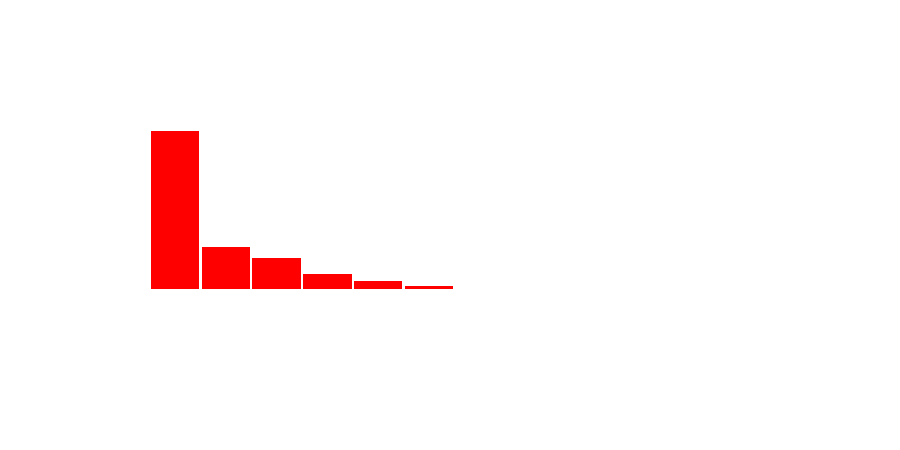
\includegraphics[scale = 0.1, clip = true, trim= 50px 60px 50px 60px]{hist-f128f3cb38588fe5202716588c047381.pdf} \\ 
  \texttt{src\_churn} & Number of lines changed (added + deleted) by the pull request. & 0.00 & 300.72 & 10.00 & 891.00 & 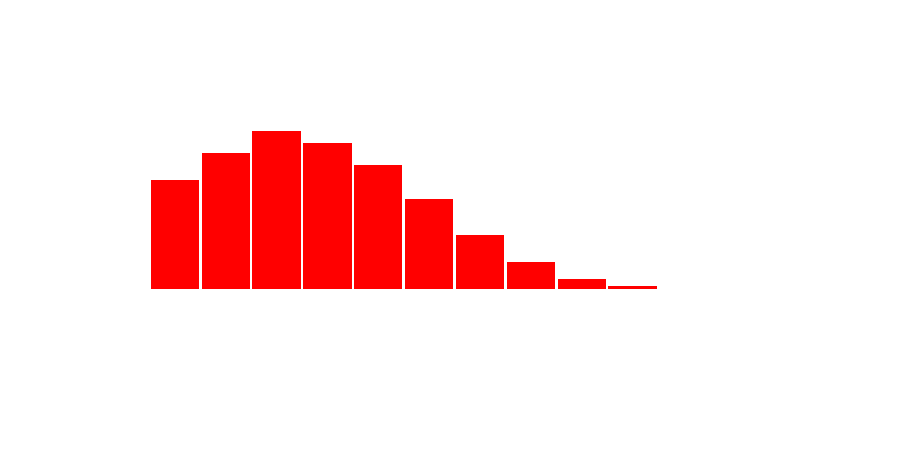
\includegraphics[scale = 0.1, clip = true, trim= 50px 60px 50px 60px]{hist-1f006c80a0da61518435a0c55f538326.pdf} \\ 
  \texttt{test\_churn} & Number of test lines changed in the pull request. & 0.00 & 88.88 & 0.00 & 282.00 & 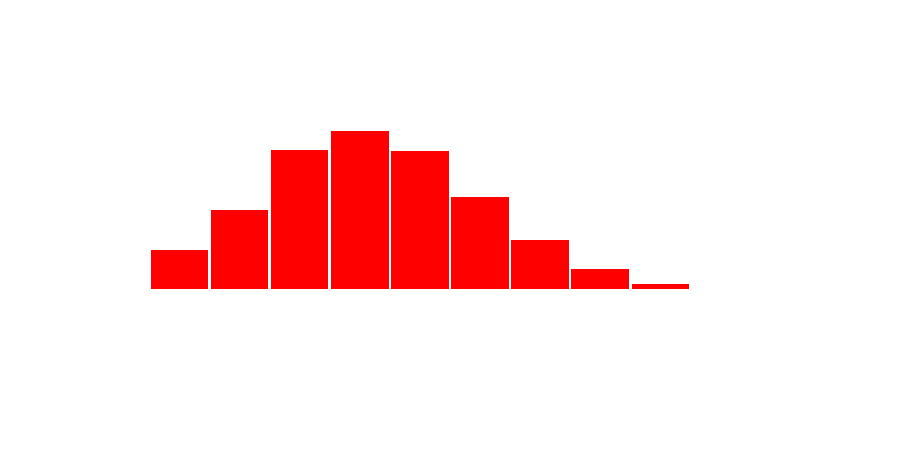
\includegraphics[scale = 0.1, clip = true, trim= 50px 60px 50px 60px]{hist-dd78ccaeedd7fc79735a66eb7f9e506b.pdf} \\ 
  \texttt{files\_changed} & Number of files touched by the pull request. & 1.00 & 12.12 & 2.00 & 31.00 & 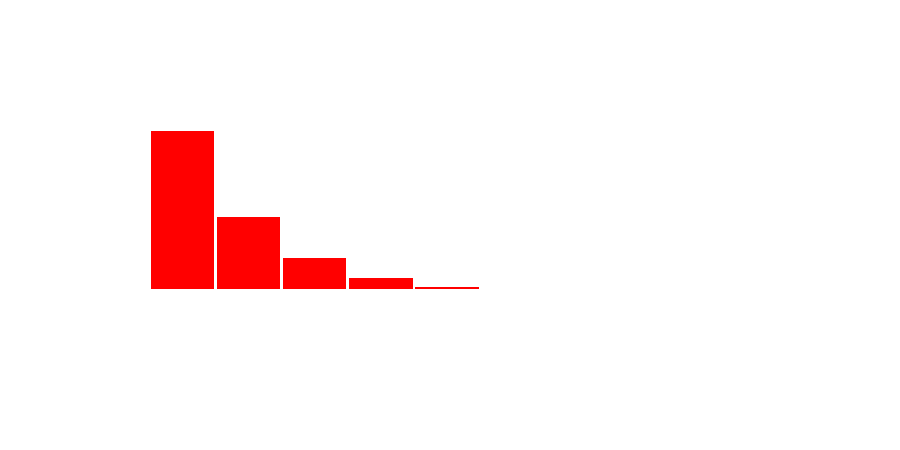
\includegraphics[scale = 0.1, clip = true, trim= 50px 60px 50px 60px]{hist-9b07b060359435635ff2bf4cd34f834a.pdf} \\ 
  \texttt{num\_comments} & The total number of comments (discussion and code review). & 0.00 & 2.77 & 1.00 & 12.00 & 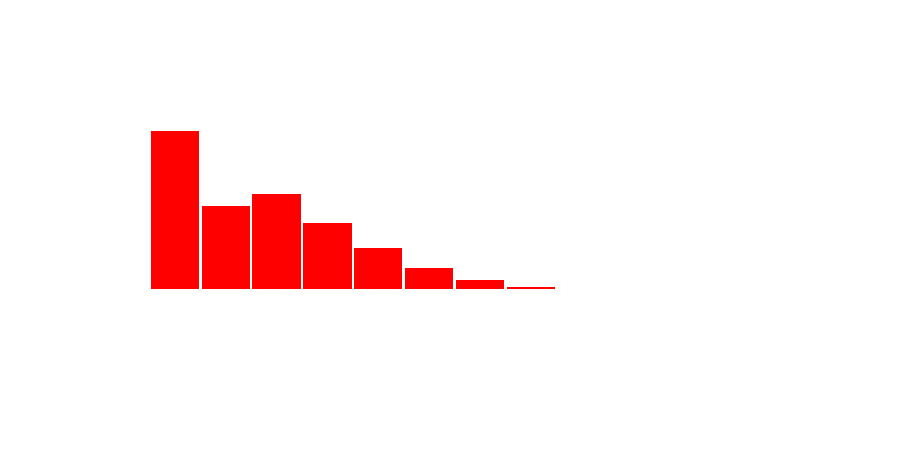
\includegraphics[scale = 0.1, clip = true, trim= 50px 60px 50px 60px]{hist-9db5e2b390de0d64d26c14798cb579ef.pdf} \\ 
  
  \texttt{conflict} & The word \emph{conflict} appears in the pull request comments.
 & --- & --- & --- & --- & ---\\

    \texttt{forward\_link} & The pull request comments include links to other
    pull requests. & --- & --- & --- & --- & --- \\


  \multicolumn{2}{l}{\bf{Project Characteristics}}\\

  \texttt{sloc} & Executable lines of code at pull request merge time. & 1,390.00 & 6,0897.87 & 26,036.00 & 302,156.00 & 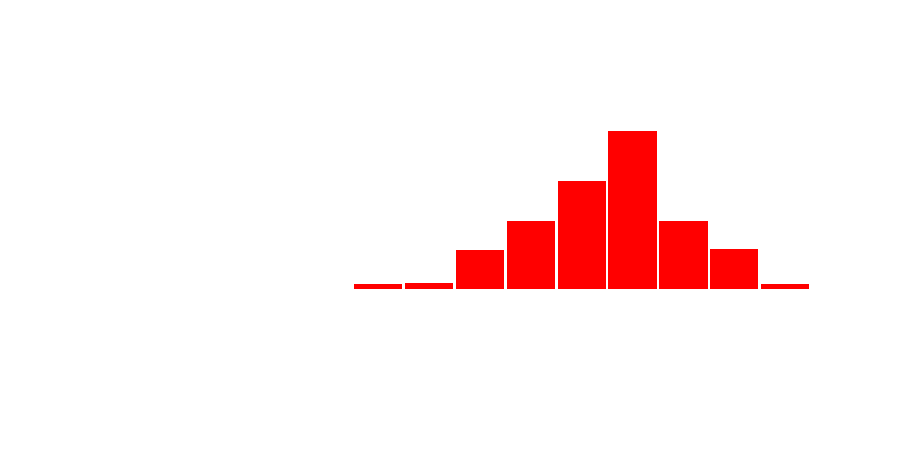
\includegraphics[scale = 0.1, clip = true, trim= 50px 60px 50px 60px]{hist-6b5159d3060b4fdf8493d4c818f79949.pdf} \\ 
  \texttt{team\_size} & Number of active core team members during the last 3 months prior to the pull request creation. & 1.00 & 15.37 & 7.00 & 65.00 & 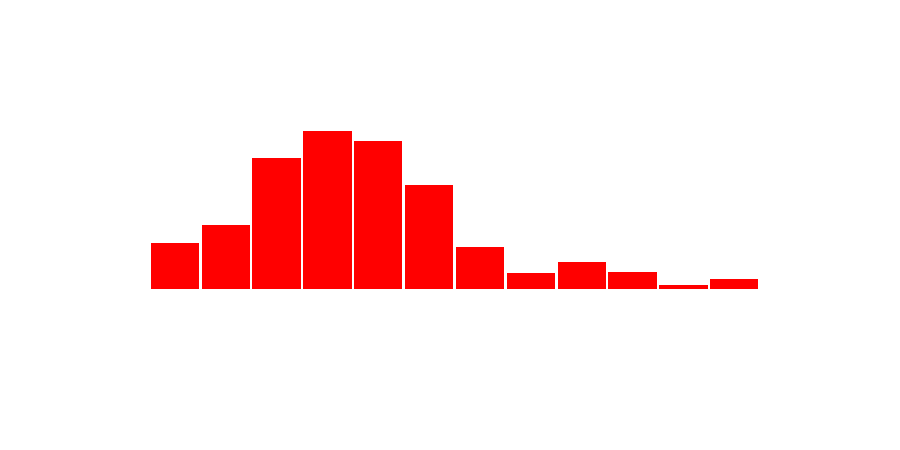
\includegraphics[scale = 0.1, clip = true, trim= 50px 60px 50px 60px]{hist-231fb4fabf4a3f0c551f2a97ae080508.pdf} \\ 
  \texttt{perc\_external\_contribs} & The ratio of commits from external members over core team members in the last 3 months prior to pull request creation. & 8.00 & 52.81 & 54.00 & 95.00 & 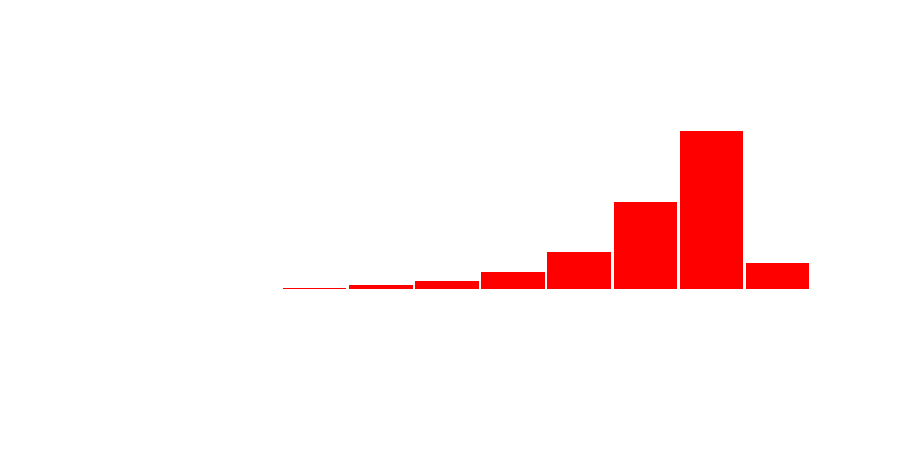
\includegraphics[scale = 0.1, clip = true, trim= 50px 60px 50px 60px]{hist-a222f0a5c377ba129dd6c8f257062591.pdf} \\ 
  \texttt{commits\_on\_files\_touched} & Number of total commits on files touched by the pull request 3 months before the pull request creation time. & 0.00 & 52.39 & 5.00 & 210.00 & 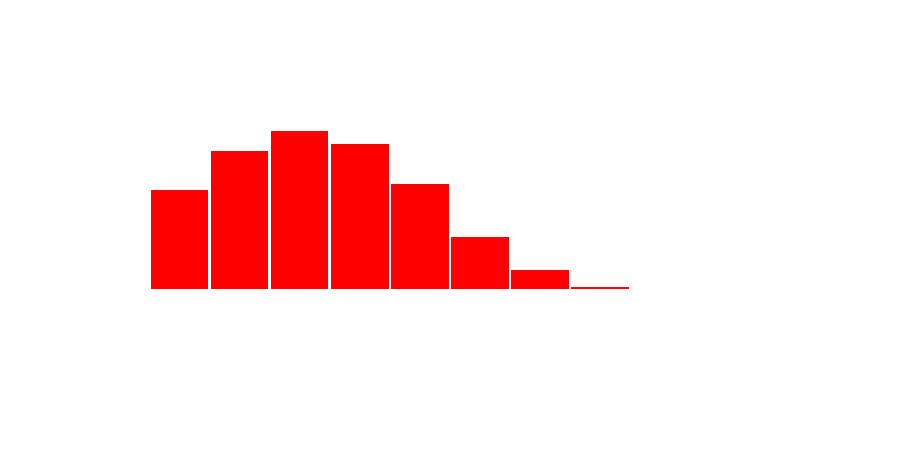
\includegraphics[scale = 0.1, clip = true, trim= 50px 60px 50px 60px]{hist-b735900ffcc37e7eda16dcd0c3497e6e.pdf} \\ 
  \texttt{test\_lines\_per\_kloc} & A proxy for the project's test coverage. & 1.39 & 1,002.61 & 440.80 & 2,147.43 & 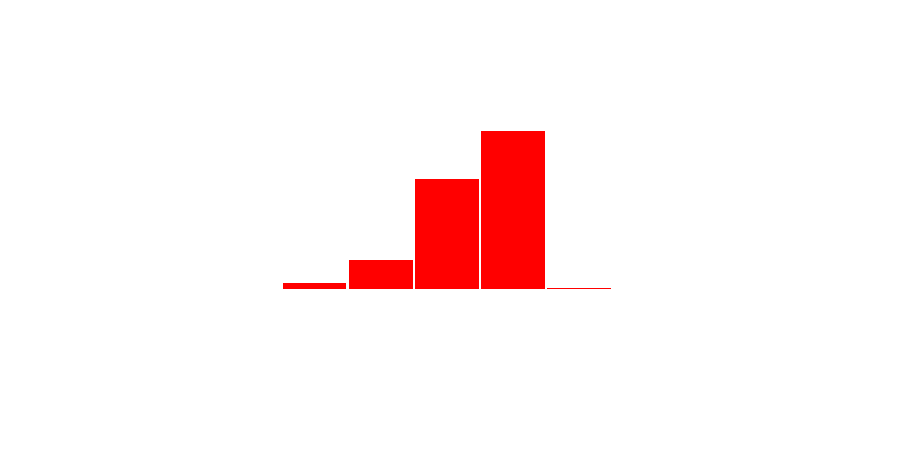
\includegraphics[scale = 0.1, clip = true, trim= 50px 60px 50px 60px]{hist-67ff3047089ba9ce0528884eab66e80a.pdf} \\ 

  \multicolumn{2}{l}{\bf{Developer}}\\

  \texttt{prev\_pullreqs} & Number of pull requests submitted by a specific developer, prior to the examined pull request. & 0.00 & 45.11 & 14.00 & 195.00 & 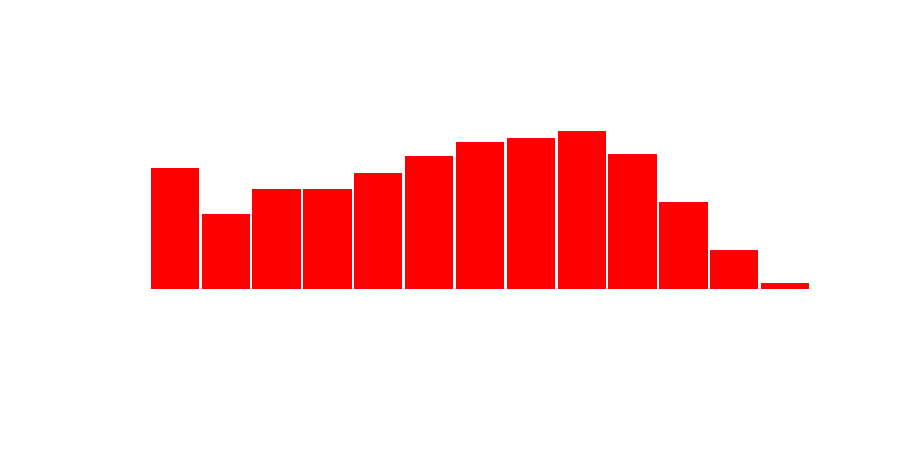
\includegraphics[scale = 0.1, clip = true, trim= 50px 60px 50px 60px]{hist-a2f7f60851dfa13cfbe0227d1d233767.pdf} \\ 
  \texttt{requester\_succ\_rate} & The percentage of the developer's pull requests that have been merged up to the creation of the examined pull request. & 0.00 & 0.59 & 0.78 & 1.00 & 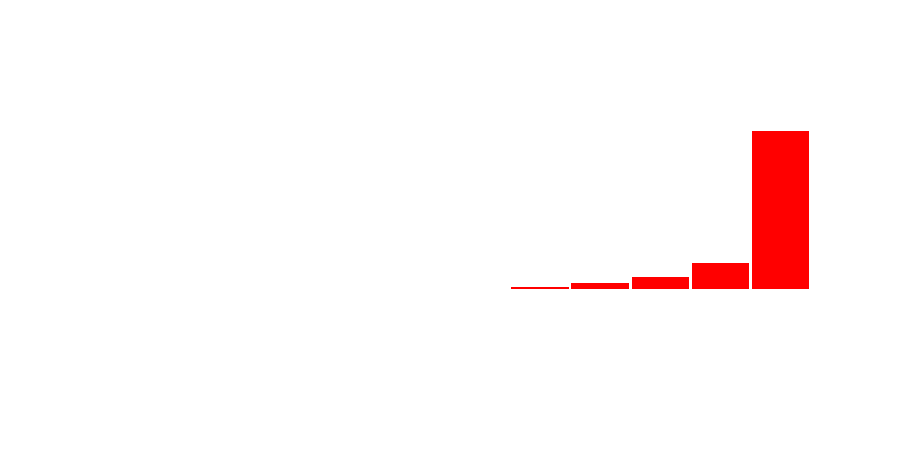
\includegraphics[scale = 0.1, clip = true, trim= 50px 60px 50px 60px]{hist-9363017165c3ded62457750f1c67c1af.pdf} \\ 
   \hline
\end{tabular}
\end{small}
\caption{Selected features and descriptive statistics. Historgrams are in log scale.} 
\label{tab:features}
\end{table*}
